\section{Probabilities}

\subsection{Basics}
The following are some basic properties of probabilities:

\noindent
Probability of an event $P(A)$

\noindent
Probability of a union of two events
\begin{equation*}
    P(A \cup B) = P(A) + P(B) - P(A \cap B)
\end{equation*}

\noindent
Conditional Probability
\begin{equation*}
    P(A | B) = \frac{P(A \cap B)}{P(B)}
\end{equation*}

\noindent
Independent events
\begin{equation*}
    P(A \cap B) = P(A) \cdot P(B)
\end{equation*}

\noindent
Bayes' rule
\begin{equation*}
    P(A|B) = \frac{P(B|A) \cdot P(A)}{P(B)}
\end{equation*}

The value of the random variable $X$ depends on the specific outcome result of stochastic events. If the range of $X$ values is discrete then it's a \textbf{discrete random variable} and if it's continuous then it's a \textbf{continuous random variable}. Probability mass function (weighted probabilities): $p_n = {\rm Pr} \{ X = x_n \}$. Note that $\sum_n p_n = 1$.

Cummulative distribution function $F(x) = {\rm Pr \{ X \in (- \infty; x] \}}$.
\begin{center}
    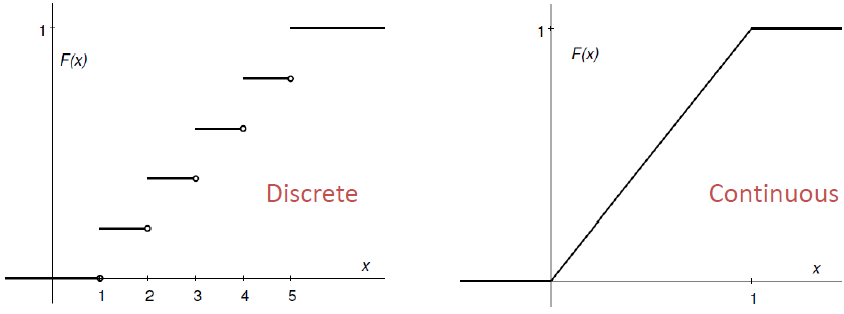
\includegraphics[width=300pt]{images/cummulative distribution function.png}
\end{center}

Probability density function $P_X = \frac{d F(x)}{dx}$, for a discrete random variable $P_X(x) = \sum_n p_n \delta(x - x_n)$. So the probability is just na integral
\begin{equation*}
    {\rm Pr} \{ a \leq X \leq b \} = \int_a^b P_X(x) dx = F(b) - F(a)
\end{equation*}

The $n$-th moment of $X$ is an expectation (mean) value of $X^n$
\begin{equation*}
    E(X^n) \equiv \langle x^n \rangle = \int x^n P_X(x) dx \quad \langle x^n \rangle = \sum_k x^n_k p_k
\end{equation*}

Expectation (mean) value
\begin{equation*}
    \mu_X = \langle x \rangle = \int x P_X(x) dx \quad \text{or} \quad \mu_X = \langle x \rangle = \sum_k x_k p_k
\end{equation*}


Mean value of a function $u(x)$
\begin{equation*}
    \langle u(X) \rangle = \int u(x) P_X(x) dx \quad \text{or} \quad \langle u(X) \rangle = \sum_k u(x_k) p_k
\end{equation*}

Note that expectation value is a linear operator.

Variance
\begin{equation*}
    \sigma_X^2 = \langle [ X - \mu_X ]^2 \rangle = \langle x^2 \rangle - \mu_X^2
\end{equation*}

\subsection*{Example: Bernoulli distribution}
Two possible values $X = \{x_0, x_1\} = \{ 0, 1\}$, with probability mass function $p_0 = q = 1 - p$ and $p_1 = p$. Then

\begin{equation*}
    \mu_x = \langle x \rangle = p \quad \text{and} \quad \sigma^2_X = \langle x^2 \rangle - \langle x \rangle^2 = p (1 - p)
\end{equation*}

\subsection{Generating functions}
Assume X is a discrete random variable $\in \mathbb{N}_0$, with probabilities

\begin{equation*}
    X = \{ 0, 1, 2, \dots \}; \quad {\rm Pr} \{ X = n\} = p_n; \quad \sum_{n=0}^{\infty} = 1
\end{equation*}

then

\begin{equation*}
    \mu_X = \sum_{n = 0}^{\infty} n p_n; \quad \sigma^2_X = \sum_{n = 0}^{\infty} n^2 p_n - \mu_X^2
\end{equation*}

The \textbf{generating function} of the random variable $X$ is defined as the following function of the real number $s$:
\begin{equation*}
    G_X(s) = \langle s^x \rangle = \sum_{n=0}^{\infty} s^n p_n
\end{equation*}
Note that the seties converges for any $|s| \leq 1$.

\begin{equation*}
    G^{\prime}_X (1) = \sum_n n p_n = \mu_X; \quad G^{\prime \prime}_X (1) = \sum_n n(n-1) p_n = \langle n^1 \rangle - \mu_X
\end{equation*}

\noindent
Also we can retrieve probabilities from the generating function

\begin{equation*}
    G_X(1) = 1 \quad G_X(0) = p_0 \quad G^{\prime}_X (0) = p_1 \quad G^{\prime \prime}_X(0) = 2!p_2 \quad \dots
\end{equation*}

For the continuous case we have
\begin{equation*}
    G_X(s) = \int P_X(x)s^x dx, \quad |s| \leq 1
\end{equation*}
Similarly, Mean value and Variance are given by
\begin{equation*}
    \mu_X = G^{\prime}_X(1) \quad \sigma_X^2 = G^{\prime \prime}_X(1) + \mu_X - [\mu_X]^2
\end{equation*}

For Independent random variables $X_1$ and $X_2$
\begin{equation*}
    G_{X_1+X_2}(s) = \langle s^{x_1 + x_2} \rangle = \langle s^{x_1} \rangle \langle s^{x_2} \rangle = G_{X_1}(s) \cdot G_{X_2} (s)
\end{equation*}

\subsection*{Example: Bernoulli distribution}
\begin{equation*}
    X=\{x_0, x_1 \} = \{0, 1\} \quad \rightarrow \quad p_n=\{ 1-p, p \}
\end{equation*}

\begin{itemize}
    \item Mean Value: $\mu_X = \langle x \rangle = p$
    \item Variance $\sigma^2_X = \langle x^2 \rangle - \mu^2_X = p (1-p) $
    \item Generating function
    \begin{equation*}
        G_X(s) = \sum_{n=0}^{1} s^n p_n = (1-p) + sp
    \end{equation*}
\end{itemize}


\subsection{Example: Uniform distribution}
Uniform discrete distribution: $X = \{1, 2, \dots, N\}$, $p_k=\frac{1}{N}$

\begin{equation*}
    \mu_X = \frac{N+1}{2} \quad \sigma_X^2 = \frac{N^2 - 1}{12}
\end{equation*}

Generating function

\begin{equation*}
    G_X(s) = \sum_{k=1}^{N} s^{k} p_k = \frac{1}{N} \sum_{k=1}^N s^k = \frac{s}{N} \frac{1 - s^N}{1 -s}
\end{equation*}

Uniform continuous distribution: $X \in [0; 1]$, $P_X(x) = 1$

\begin{equation*}
    \mu_X = \frac{1}{2}, \quad \sigma^2_X = \frac{1}{12}
\end{equation*}

\begin{equation*}
    G_X(s) = \int_{0}^{1} s^x dx = \frac{s - 1}{\ln s}
\end{equation*}


\subsection*{Example: Binomial distribution}
Assume a population of $N$ bacteria, each of them can be either alive (with probability $p$) or dead (with probability $1-p$)

Let $Y = \{0, 1, 2, \dots \}$ be the number of alive bacteria, then
\begin{equation*}
    p_k = \frac{N!}{k! (N-k)!} p^k (1-p)^{N-k}
\end{equation*}

Note that $Y = X_1 + X_2 + \dots + X_N$, where $X_j$ are independent Bernoulli's variables, then this makes it easier to compute the generating function

\begin{equation*}
    G_Y(s) = [G_{X_1}(s)]^N = [1-p+sp]^N
\end{equation*}

Then mean value and variance are just
\begin{equation*}
    \mu_Y = G^{\prime}_Y(1) = Np \quad \text{and} \quad \sigma^2_Y = G^{\prime \prime} + \mu_Y - \mu^2_Y = Np(1-p)
\end{equation*}


\subsection*{Example: Poisson distribution}
It corresponds to the binomial distribution in the limit $N \rightarrow \infty$, $p \rightarrow 0$, with the product $N p = \lambda = {\rm const}$.

\begin{equation*}
    p_k = \frac{\lambda^{k e^{-\lambda}}}{k!}
\end{equation*}

Generating function
\begin{equation*}
    G_X(s) = \sum^{\infty}_{k=0} s^k p_k = e^{- \lambda} \sum^{\infty}_{k=0} \frac{(s \lambda)^k}{k!} = \exp(\lambda(s-1))
\end{equation*}

Again the mean value and variance can be easily obtained
\begin{equation*}
    \mu_X = G^{\prime}(1) = \lambda \quad \text{and} \quad \sigma_X^2 = G^{\prime \prime}_X(1) + \mu_X - \mu_X^2 = \lambda
\end{equation*}

\subsection*{Exponential distribution}
The distribution of the delay times until some event is usually described by the exponential law:

\begin{equation*}
    X \in [0; \infty), \quad P_X(x) = \lambda e^{- \lambda x},
\end{equation*}

\begin{equation*}
    \mu_X = \int_{0}^{\infty} \lambda x e^{- \lambda x} dx = \frac{1}{\lambda} \quad \sigma_X^2 = \int_{0}^{\infty} \lambda x^2 e^{- \lambda x} dx - \mu^2_X = \frac{1}{\lambda^2}
\end{equation*}


\subsection*{Example: Normal (Gaussian) distribution}
\begin{equation*}
    X \in (-\infty; \infty), \quad P_X(x) = \frac{1}{\sigma \sqrt{2 \pi}} \exp^{-\frac{(x-\mu)^2}{2 \sigma^2}}
\end{equation*}

\begin{equation*}
    \mu_X = \mu \quad \sigma_X^2 = \sigma^2
\end{equation*}


\subsection{Stochastic processes}
A stochastic process us sycga oricessm when the value of the random variable $X$ changes with time. Assume that at some specific time moments $t_1$, $t_2$, $t_3$ ... the random variable $X$ acquired values $X_1$, $X_2$ and so on respectively. Then the multi-variable probability density function $P(X_1, t_1; X_2, t_2; \dots)$. And the conditional probability

\begin{equation*}
    P(X_1, t_1; X_2, t_2; \dots | X_1^{\prime}, t_1^{\prime}; X_2^{\prime}, t_2^{\prime}; \dots) = \frac{P(X_1^{\prime}, t_1^{\prime}; X_2^{\prime}, t_2^{\prime}; \dots; X_1, t_1; X_2, t_2; \dots)}{P(X^{\prime}_1, t^{\prime}_1; X^{\prime}_2, t_2^{\prime}; \dots )}
\end{equation*}

The Markov chain is a stochastic process \textit{without memory} meaning

$P(X_1; t_1; X_2, t_2; \dots | X_1^{\prime}, t^{\prime}_1)$

Thus for some time series

\begin{equation*}
    P(X_1, t_1; X_2, t_2; \dots X_n, t_n) = \prod_{k=1}^{n} P(X_k, t_k | X_{k-1} t_{k-1})
\end{equation*}

If the one-step probability does not depend on time, the process is called the stationary (or time-homogeneous) Markoc-Chain:
\begin{equation*}
    P(X_2, t_2 | X_1, t_1) = p_{21}
\end{equation*}
Where $\sum_j p_{ji} = 1$ and $p_{ji} > 0$

\subsection*{Example: Two species}
Suppose there is a forest, where only two species of trees can grow - say, A and B. with similar growing rate and lifetime.

In general each generation, every old tree is replaced with a new young tree of either the same or different species. This is discrete-time Markov process, where time $t_n$ represents the $n$-th generation

\begin{center}
    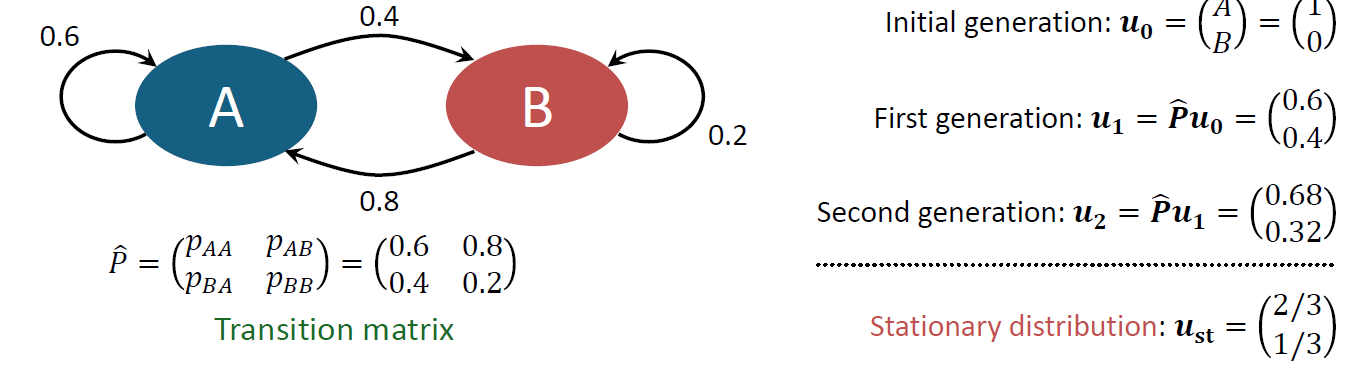
\includegraphics[width=300pt]{images/two species example.png}
\end{center}